\documentclass[12pt,-letter paper]{article}
\usepackage{siunitx}
\usepackage{setspace}
\usepackage{gensymb}
\usepackage{xcolor}
\usepackage{caption}
%\usepackage{subcaption}
\doublespacing
\singlespacing
\usepackage[none]{hyphenat}
\usepackage{amssymb}
\usepackage{relsize}
\usepackage[cmex10]{amsmath}
\usepackage{mathtools}
\usepackage{amsmath}
\usepackage{commath}
\usepackage{amsthm}
\interdisplaylinepenalty=2500
%\savesymbol{iint}
\usepackage{txfonts}
%\restoresymbol{TXF}{iint}
\usepackage{wasysym}
\usepackage{amsthm}
\usepackage{mathrsfs}
\usepackage{txfonts}
\let\vec\mathbf{}
\usepackage{stfloats}
\usepackage{float}
\usepackage{cite}
\usepackage{cases}
\usepackage{subfig}
%\usepackage{xtab}
\usepackage{longtable}
\usepackage{multirow}
%\usepackage{algorithm}
\usepackage{amssymb}
%\usepackage{algpseudocode}
\usepackage{enumitem}
\usepackage{mathtools}
%\usepackage{eenrc}
%\usepackage[framemethod=tikz]{mdframed}
\usepackage{listings}
%\usepackage{listings}
\usepackage[latin1]{inputenc}
%%\usepackage{color}{   
%%\usepackage{lscape}
\usepackage{textcomp}
\usepackage{titling}
\usepackage{hyperref}
%\usepackage{fulbigskip}   
\usepackage{tikz}
\usepackage{graphicx}
\lstset{
  frame=single,
  breaklines=true
}
\let\vec\mathbf{}
\usepackage{enumitem}
\usepackage{graphicx}
\usepackage{siunitx}
\let\vec\mathbf{}
\usepackage{enumitem}
\usepackage{graphicx}
\usepackage{enumitem}
\usepackage{tfrupee}
\usepackage{amsmath}
\usepackage{amssymb}
\usepackage{mwe} % for blindtext and example-image-a in example
\usepackage{wrapfig}
\title{CIRCLES}
\author{Arvind Kumar}
\date{Dec 2023}
\begin{document}
\maketitle
\begin{enumerate}
	\item In \figref{fig:Figure1}, from an external point $P$, two tangent $PQ$ and $PR$ are drawn to a circle of radius $4cm$ with center $O$. If$\angle{PQR}=90\degree$, then length of $PQ$ is \underline {\hspace{4cm}}.
\begin{enumerate}[label=(\alph*)]
\item $3cm$ 
\item $4cm$
\item $2cm$
\item $2{\sqrt{2}}cm$ 
\end{enumerate}
\begin{figure}[H]
\centering
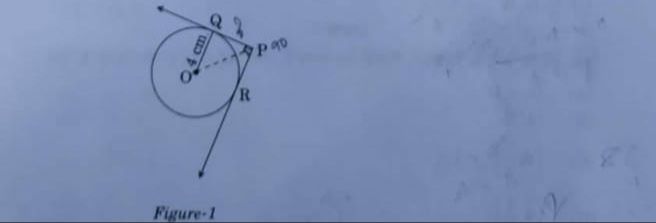
\includegraphics[width=\columnwidth]{Figs/file1.jpg}
\caption{Circle with intersecting line and external points}
\label{fig:Figure1}
\end{figure}
\item In \figref{fig:Figure2}, $PQ$ is tangent to the circe with center at $O$, at the point $B$. If$\angle{AOB}=100\degree$, then$\angle{ABP}$ is equal to\newline
\begin{enumerate}[label=(\alph*)] 
\item $50\degree$ 
\item $40\degree$ 
\item $60\degree$ 
\item $80\degree$
\end{enumerate}
\begin{figure}[H]
\centering
\includegraphics[width=\columnwidth]{Figs/file2.jpg}
\caption{Geometric Diagram}
\label{fig:Figure2}
\end{figure}
\item In \figref{fig:Figure3}, quadrilateral $ABCD$ is drawn to circumscribe a circle. Prove that\newline
$AB+CD=BC+AD$
\begin{figure}[H]
\centering
\includegraphics[width=\columnwidth]{Figs/file3.jpg}
\caption{Inscribed Circle in a Rectangle}
\label{fig:Figure3}
\end{figure}
\item In \figref{fig:Figure4}, find the perimeter of $\triangle ABC$, if $AP=12cm$
\begin{figure}[H]
\centering
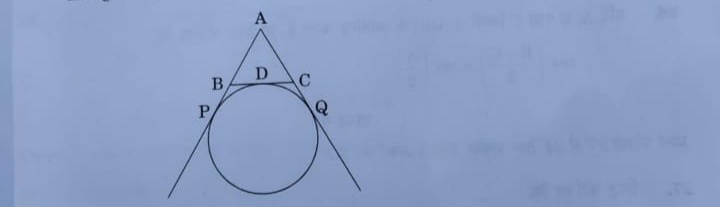
\includegraphics[width=\columnwidth]{Figs/file4.jpg}
\caption{Inscribed Triangle in a Triangle}                                                   
\label{fig:Figure4}
\end{figure}
\end{enumerate}
\end{document}
